%%%%%%%%%%%%%%%%%%%%%%%%%%%%%%%%%%%%%%%%%%%%%%%%%%%%%%%%%%%%%%%%%%%
%                                                                 %
%                            CHAPTER ONE                          %
%                                                                 %
%%%%%%%%%%%%%%%%%%%%%%%%%%%%%%%%%%%%%%%%%%%%%%%%%%%%%%%%%%%%%%%%%%%

\chapter{INTRODUCTION} \label{sec:introduction}

How many plains zebras (\textit{Equus quagga}) and Masai giraffes (\textit{Giraffa camelopardalis tippelskirchi}) are in the Nairobi National Park?

The question, at its surface, may seem trivial -- a two year old child can reliably count zebras and giraffes -- but the answer becomes difficult to obtain when the population becomes unmanageable.  To be more precise, the unmanageability originates when either the conservation area is too large to be effectively and efficiently sampled, the population grows to a point that exceeds the conservationists' ability to keep reliable records of the different individuals, or both.  At that point, finding the answer becomes intractable for human-powered identification and analysis.  For the Nairobi National Park, the problem is further complicated by the fact that the park is not fenced on its southern side -- it is typical of most conservancies in Kenya to have an unfenced boundary to prevent limiting natural migration -- making the actual zebra and giraffe population arbitrary at any particular moment, and ever-changing.  Therefore, merely locating the zebras within the park and producing a representative sampling of the population is a significant obstacle.

%\begin{figure*}[t]%
\begin{figure}[!htb]%
    \centering
    \subfloat[]{{ $\vcenter{\hbox{ 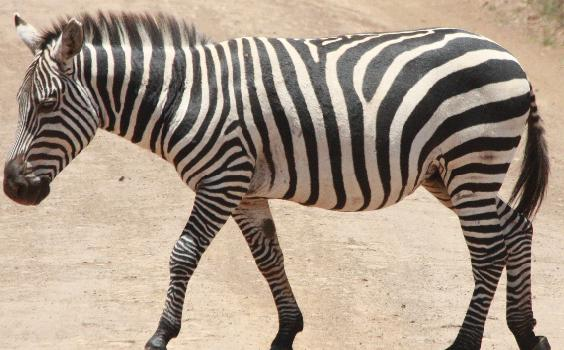
\includegraphics[width=0.215\textwidth]{resources/matching/1-667-2.jpeg} }}$ }}%
    \subfloat[]{{ $\vcenter{\hbox{ 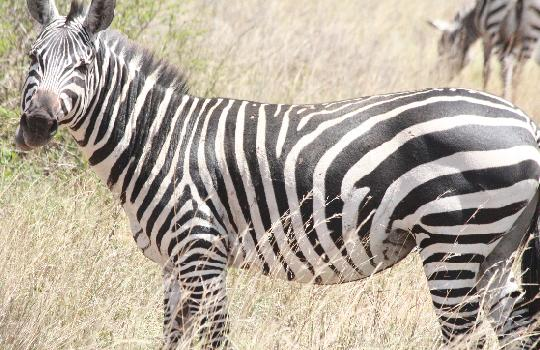
\includegraphics[width=0.215\textwidth]{resources/matching/10-229-1.jpeg} }}$ }}%
    \subfloat[]{{ $\vcenter{\hbox{ 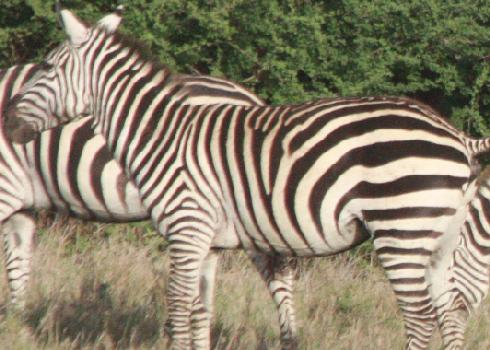
\includegraphics[width=0.215\textwidth]{resources/matching/11-253-2.jpeg} }}$ }}%
    \subfloat[]{{ $\vcenter{\hbox{ 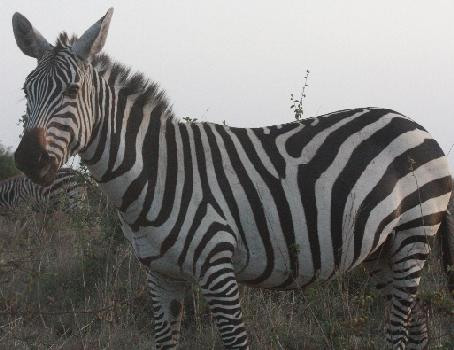
\includegraphics[width=0.215\textwidth]{resources/matching/12-2773-2.jpeg} }}$ }}%
    \vspace{0.1cm}
    \subfloat[]{{ $\vcenter{\hbox{ 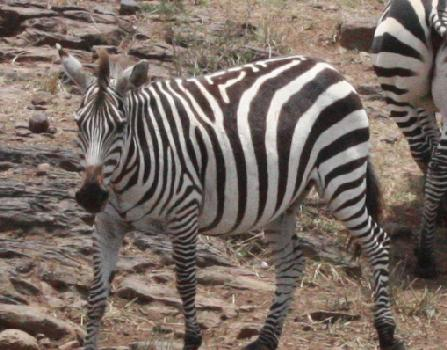
\includegraphics[width=0.215\textwidth]{resources/matching/13-3039-2.jpeg} }}$ }}%
    \subfloat[]{{ $\vcenter{\hbox{ 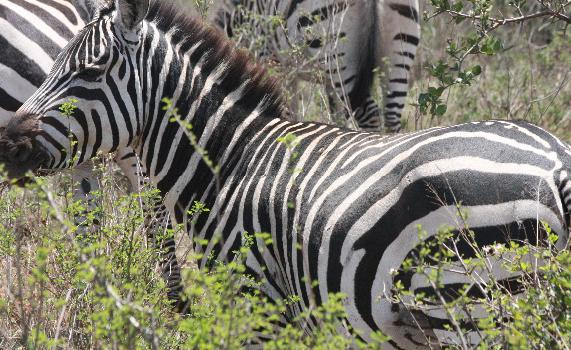
\includegraphics[width=0.215\textwidth]{resources/matching/14-229-2.jpeg} }}$ }}%
    \subfloat[]{{ $\vcenter{\hbox{ 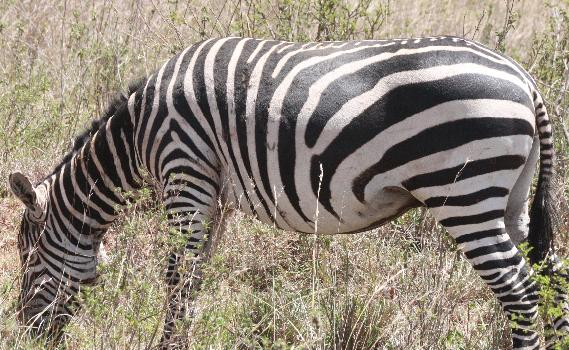
\includegraphics[width=0.215\textwidth]{resources/matching/15-236-1.jpeg} }}$ }}%
    \subfloat[]{{ $\vcenter{\hbox{ 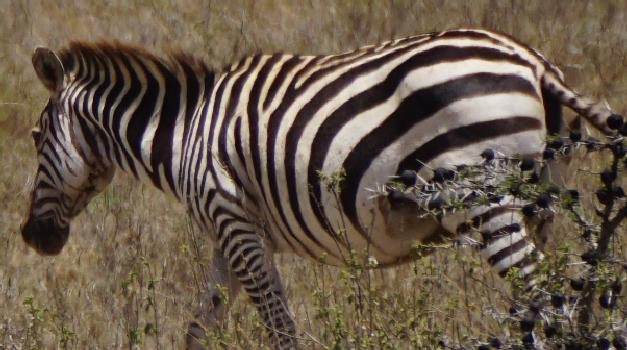
\includegraphics[width=0.215\textwidth]{resources/matching/16-3039-1.jpeg} }}$ }}%
    \vspace{0.1cm}
    \subfloat[]{{ $\vcenter{\hbox{ 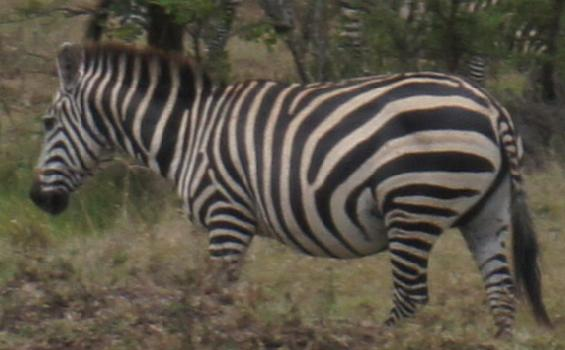
\includegraphics[width=0.215\textwidth]{resources/matching/17-3250-2.jpeg} }}$ }}%
    \subfloat[]{{ $\vcenter{\hbox{ 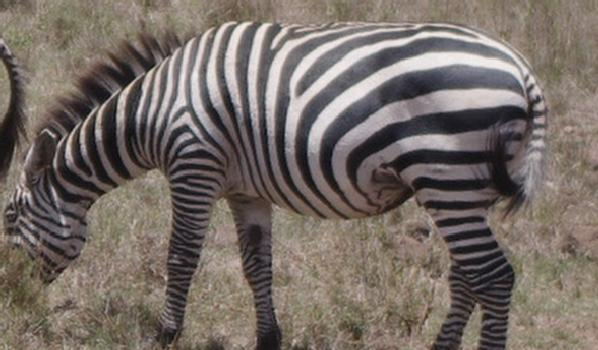
\includegraphics[width=0.215\textwidth]{resources/matching/18-667-1.jpeg} }}$ }}%
    \subfloat[]{{ $\vcenter{\hbox{ 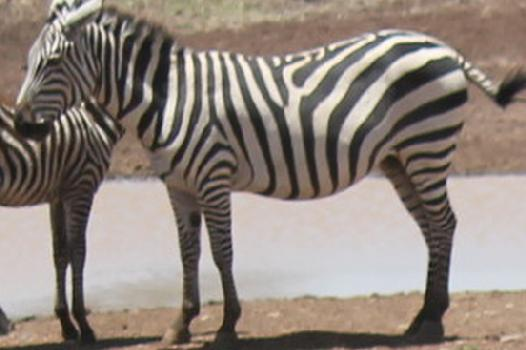
\includegraphics[width=0.215\textwidth]{resources/matching/19-2773-1.jpeg} }}$ }}%
    \subfloat[]{{ $\vcenter{\hbox{ 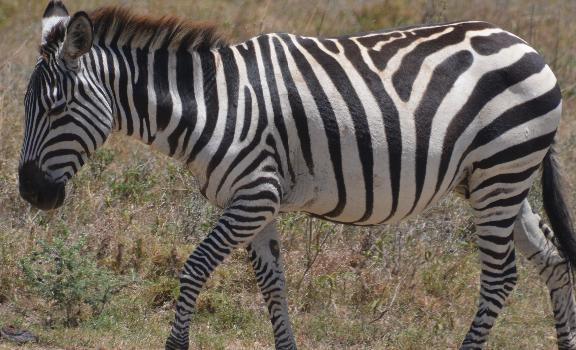
\includegraphics[width=0.215\textwidth]{resources/matching/2-56-1.jpeg} }}$ }}%
    \vspace{0.1cm}
    \subfloat[]{{ $\vcenter{\hbox{ 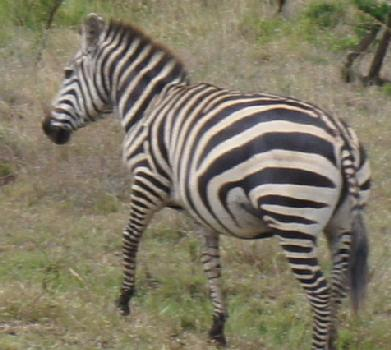
\includegraphics[width=0.215\textwidth]{resources/matching/20-3250-1.jpeg} }}$ }}%
    \subfloat[]{{ $\vcenter{\hbox{ 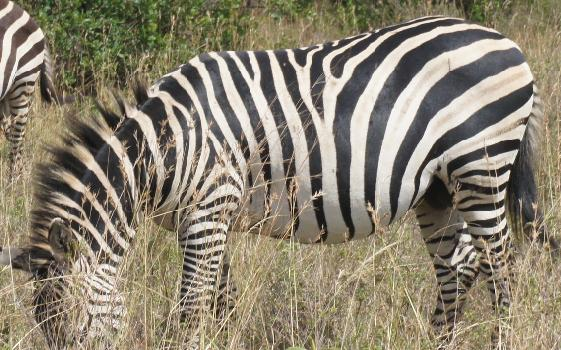
\includegraphics[width=0.215\textwidth]{resources/matching/3-212-1.jpeg} }}$ }}%
    \subfloat[]{{ $\vcenter{\hbox{ 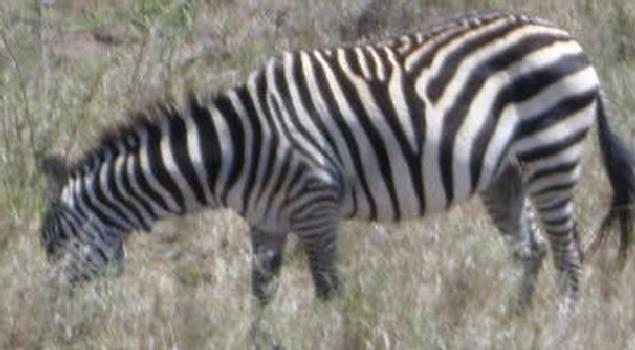
\includegraphics[width=0.215\textwidth]{resources/matching/4-253-1.jpeg} }}$ }}%
    \subfloat[]{{ $\vcenter{\hbox{ 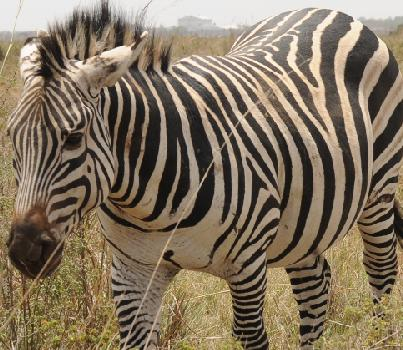
\includegraphics[width=0.215\textwidth]{resources/matching/5-212-2.jpeg} }}$ }}%
    \vspace{0.1cm}
    \subfloat[]{{ $\vcenter{\hbox{ 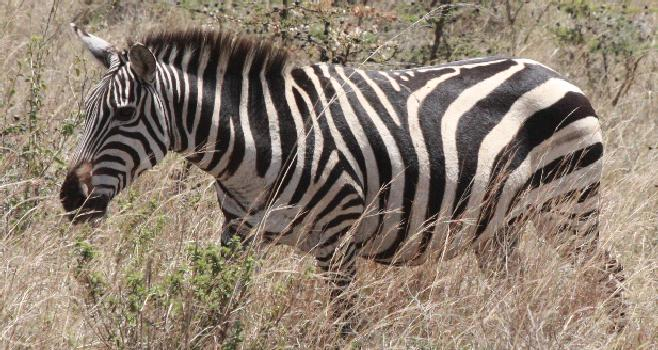
\includegraphics[width=0.215\textwidth]{resources/matching/6-583-1.jpeg} }}$ }}%
    \subfloat[]{{ $\vcenter{\hbox{ 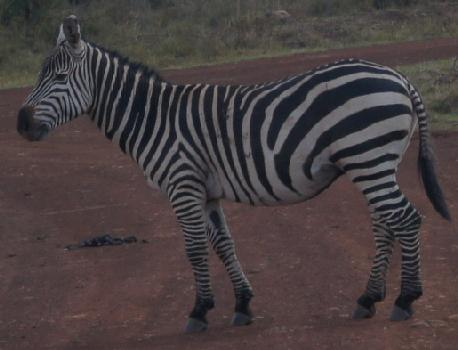
\includegraphics[width=0.215\textwidth]{resources/matching/7-236-2.jpeg} }}$ }}%
    \subfloat[]{{ $\vcenter{\hbox{ 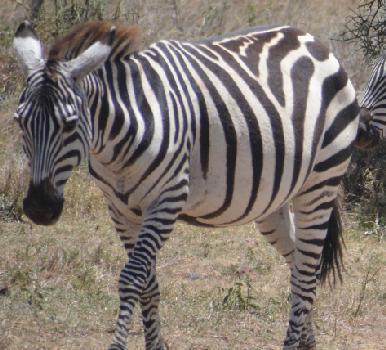
\includegraphics[width=0.215\textwidth]{resources/matching/8-56-2.jpeg} }}$ }}%
    \subfloat[]{{ $\vcenter{\hbox{ 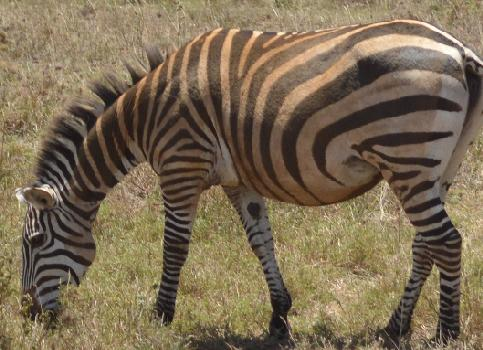
\includegraphics[width=0.215\textwidth]{resources/matching/9-583-2.jpeg} }}$ }}%
    \vspace{0.1cm}
    \caption[Matching Game for Pairs of 10 Individual Zebras]{\textbf{Matching Game for Pairs of 10 Individual Zebras.}  A game to match the pairs (2 images per animal) of 10 identified individuals seen during the GZGC.    Answers can be found in Table \ref{tab:answers} in the Appendix.  Once completed, we suggest the reader reflect on the follwing questions: 1) ``How confident are you in your matches?'' 2) ``How difficult was the appearance-based matching?'' 3) ``How long did it take?'' and 4) Using the answers, ``How accurate were your matches?''}
        \label{fig:matching}
\end{figure}

The intractability is not as much of a concern for larger or endangered species such as elephants and rhinoceroses, where a small, local population can be manageably and reliably identified using ear notches and tags \cite{mukinya_identification_1976}, radio collars \cite{alexander_african_1994, mech_critique_2002, thouless_long_1995}, or other physical distinguishing features (e.g.\ deformities, scars, face shape, ear shape and wrinkles) \cite{patrick_demographic_2003, sikes_guidelines_2011}.   However, most of these approaches are \textit{invasive} and require involved procedures, such as incapacitating the animal using expensive tranquilizers and employing experienced veterinarians.  A better approach to estimating the animal population would be to simply use the appearance of the animal to \textit{passively} (non-invasively) identify the individual.  For large populations of zebra or giraffe, or even large populations of elephant or rhinoceros, the cost and demanding logistics makes invasively identifying the population infeasible.  Therefore, a passive, appearance-based approach is preferred.  However, it is exceedingly difficult for humans to reliably distinguish between different individual animals based solely on unaltered appearance \cite{crall_hotspotter_2013} without added identifying markers.  To illustrate this, we have provided an example of 20 images of zebras in Figure \ref{fig:matching}.  We invite the reader to spend (at most) 10 minutes examining and to attempt matching the image pairs (2 images per animal) for 10 identified individuals.  These sightings of zebra were selected from the population at the Nairobi National Park.  The purpose of the matching game is to highlight the uncertainty, difficulty, and duration of matching between different sightings of zebras.  For brevity, the discussion in this thesis will focus largely on plains zebras since the procedure and concepts are identical between zebras and giraffes.  We will revisit Masai giraffes in Chapter \ref{sec:results}.

Despite these challenges, it is still important for the conservationists to have an accurate estimate of the zebra population within the park.  Knowing the number of zebras can be used to measure the overall health of the park's ecosystem and can be used to help answer ecological questions, such as: ``is the population stable and self-sustaining?''\ \cite{andersen_population_2015, boyce_population_1992, coulson_use_2001, macedo_ecology_2010}, ``what are the population's age and sex demographics?''\ \cite{romer_population_2015, macedo_ecology_2010}, ``what is the life-expectancy?''\ \ \cite{romer_population_2015, macedo_ecology_2010, white_program_1999}, ``what is the impact of the population on the park's environment?''\ \cite{keesing_impacts_1998, macedo_ecology_2010}, and -- with GPS data -- ``what are the migratory patterns and locations of concentration?''\ \cite{karanth_estimating_2012, subedi_population_2013}.  The answers to these questions can be used by the conservationists to make data-driven decisions to better coordinate and focus their conservation efforts.  Up until now, estimates of the population in the Nairobi National Park were performed by simply counting sighted individuals within sub-sections of the park on a given day (e.g.\ \cite{oconnell_abundance_2011, seber_estimation_1982, subedi_population_2013}) or by counting from aerial surveys (e.g.\ \cite{caughley_sampling_1977, melville_aerial_2008, zero_monitoring_2013}). These counting-based procedures are prone to errors such as double counting, under-sampling, and sampling bias \cite{buckland_quantifying_1991, graham_investigating_1989, jachmann_comparison_2002, jolly_problem_1983, robson_sample_1964}.  A better system for producing a population estimate is therefore desired.  In this thesis, we present an alternate population counting method by implementing a distributed, automated, appearance-based approach to address these challenges and ultimately provide conservationists with the data they require.

To address the difficulty of sampling a large population and having to survey a large conservation area, we propose employing the help of volunteer participants.  The volunteers are tasked with photographing every zebra they encounter in an assigned zone (sub-section) within the conservation area, which provides input to a computer vision algorithm.  It is important to note that while the scientific contributions of these volunteers can be critical to a population estimate, the process should also be engaging and rewarding for these participants.  These so-called \textit{citizen scientists} \cite{cohn_citizen_2008, haklay_geographical_2010, sui_citizen_2013, irwin_citizen_1995, silvertown_new_2009} can be deputized for data collection and can thus significantly reduce the demands of performing a park-wide population monitoring study, freeing logistical man-power for other administrative duties.  If a large sampling of images is obtained, the challenge of estimating the zebra population is reformulated from an individual, human-powered identification and analysis problem into a highly-distributed, semi-automated, appearance-based process that uses images contributed by citizen scientists as input.  It should be mentioned that compared to camera traps, trail cameras, and automated camera drones, enlisting the help of citizen scientists is logistically simpler (e.g.\ no need to setup, monitor, and retrieve cameras) and obviously does not require purchasing additional hardware.  The images taken by a human photographer are generally of superior quality since a volunteer can be trained to take only useful pictures.  These benefits, however, come at the cost of having to incentivize citizen scientist involvement.   The involvement of citizen scientists also introduces sampling biases (e.g.\ trail cameras and camera traps capture images during night whereas volunteers might not).  An unbiased population monitoring study should use many sources of image input as can be reasonably obtained, however we only utilized images taken by citizen scientists for our sampling.

To address the inaccuracies and inefficiencies of human-powered, appearance-based identification, we propose leveraging the computational power of computer vision algorithms to help with tedious and high-volume tasks.  The computer vision algorithms are a starting point for beginning to automatically answer the following questions:
\begin{enumerate}
    \item Given an image, where are all of the zebras located?  % The computer vision answer is object detection and localization.
    \item Given a sighting of a zebra, is it of sufficient quality (e.g.\ exposure, focus, etc.)\ for identifying that individual?  % The computer vision answer is using scene features (GIST descriptors)
    \item Given a sighting of a zebra, how does its appearance describe that individual's identity?  Furthermore, is the description of sufficient quality to recognize that individual in the future?  % The computer vision answer is feature extraction.
    \item Given a zebra's description, has that individual zebra ever been seen previously?  % The computer vision answer is object recognition.
\end{enumerate}
The computer vision algorithms used in this thesis offer enough aid to make passive, appearance-based population monitoring feasible for large populations.

In the past, tedious appearance-based techniques were developed for estimating the size of an animal population.  Starting in the 1980's, film photographs were taken of animals and developed on-location to produce image negatives.  Using the negatives, the animal's stripes and visual patterns were traced onto paper by hand and a location-specific bifurcation tree was generated for identifying the known individuals  \cite{ginsberg_social_1988}.  This process was very resource intensive, had problems scaling to larger populations, and relied heavily on taking clear images from fixed viewpoints.  In the mid-1990's, software solutions for indexing the population began to emerge.  Using the encoding method described by Ginsberg \cite{ginsberg_social_1988}, the appearance of the animal was encoded into a (mostly) deterministic and searchable identification tag.  To query an animal, a regular expression search was used to find matching candidate images that were associated with a similar identification tag.  While much faster than the previous method, errors in determining the identification tag made the system difficult to use without rather extensive biological experience.  In the early 2000's, software developed by Hiby et al.  \cite{hiby_computer_1990, hiby_analysis_2013} allowed for a more sophisticated identification database to be created using visual \textit{guide dots}, which further improved the accuracy of searching but the required annotating of the algorithm's features was labor-intensive and slow.  As faster computers and more advanced computer vision algorithms became available, new algorithms (e.g.\ StripeSpotter \cite{lahiri_biometric_2011} and HotSpotter \cite{crall_hotspotter_2013}) succeeded in reducing or eliminating the amount of manual annotation required before performing a search in an identification data structure.  Our overall approach is very similar in structure and technical application to the work of Bolger et. al. \cite{bolger_computer-assisted_2012}, which was a computer-assisted ``photographic mark-recapture'' technique developed independently of our system.  Their culminating interface, called \texttt{Wild-ID}, and overall algorithm (while less sophisticated than our current software prototype) still achieved impressive results for Masai giraffes in northern Tanzania.

Previously, the most current and accurate population estimates for the zebra and giraffe populations in the Nairobi National Park were based on \textit{counting} methods.  In contrast, the population estimate described in this thesis is based on performing a \textit{photographic censusing}, or photographic mark-recapture (PMR)\cite{bolger_computer-assisted_2012} study, of the population.  The primary difference between counting and photographic censusing is that counting does not take into consideration resighted animals nor does it have the capability to capture fine-grained ecological data for individuals within the population (e.g.\ life-expectancy, individual movement, etc.).  A photographic censusing of the population, however, is able to recognize a resighted animal based on its appearance and produce more accurate ecological statistics for that individual and the population as a whole.  The most recent population count (2011) based on counting methods for plains zebras in the Nairobi National Park estimated 1000 - 2000 individuals and 100 individuals for Masai giraffes \cite{ogutu_changing_2013}.  While these estimates were performed annually or semi-annually, they do not provide continuous information, are a logistical and financial burden on the park administrators, and - since they do not capture individual-level information - do not accurately account for population changes due to birth, death, migration, or immigration.  One of the main contributions of this paper is to provide an appearance-based census of the zebra and giraffe populations within the Nairobi National Park which is robust by monitoring the sightings of individual animals over time.

In March of 2015, we administered a two-day data collection event entitled \textit{The Great Zebra \& Giraffe Count} (GZGC) during the \textit{Kenya Wildlife Festival} in Nairobi, Kenya.  The GZGC employed the help of volunteer citizen scientists to help collect image data and was powered by the IBEIS computer vision system; IBEIS is a Python-based, computer vision pipeline, based on the HotSpotter \cite{crall_hotspotter_2013} recognition algorithm.  During the GZGC, IBEIS semi-automatically\footnote{meaning it automatically offered weighted results that had to be reviewed} localized the animal in the image, filtered detections based on quality, described the animal, used the description to build and search a database for potential matches, verified the matches, aggregated the matches into a final weighted score, and semi-automatically used the final score to decide if the animal has been seen previously \cite{gall_class-specific_2009, lowe_distinctive_2004, muja_fast_2009}.  To our knowledge, this is the first time a population estimate of the plains zebras and Masai giraffes \footnote{IBEIS is designed to process many different species and is not limited to just zebras or giraffes.} has ever been performed using an automated appearance-based approach.  We also believe that the GZGC was the largest citizen science data collection event ever performed inside the park, to date.

This thesis describes the technical aspects of the citizen science data collection and the resulting analysis generated by using a prototype version of IBEIS.  Since the IBEIS prototype was incomplete, and the volume of data contributed during the GZGC was large, we needed to develop additional interfaces for efficient image submission and distributed reviewing of the results generated by the computer vision algorithms.  We also developed several innovative computer vision algorithms to replace human-powered annotating with automated tools for the next version of IBEIS and future population counting events.  The remaining chapters of this thesis describe the specific details of our approach used during the GZGC and the results, as follows.  Chapter \ref{sec:collection} describes the data collection and citizen scientist participation.  Chapter \ref{sec:analysis} details the analysis performed on the collected data using IBEIS.  Chapter \ref{sec:verification} covers the verification performed on the analysis.  Chapter \ref{sec:results} reports the results and the estimated zebra population in the park.  Finally, Chapter \ref{sec:conclusion} summarizes our results and concludes by giving future suggestions for improvements.

As a final introductory comment, we note that IBEIS is a large and complex system, with many contributors, and is far too expansive to comprehensively describe in a single Master's thesis.  Therefore, this thesis focuses on the author's current -- and somewhat-disjoint -- contributions to IBEIS and its usage during the GZGC.  Future Ph.D. dissertations will describe the major computer vision contributions and detailed aspects of the full IBEIS computer vision architecture.

\paragraph{Terminology}
We will refer to the Nairobi National Park as NNP, \textit{The Great Zebra \& Giraffe Count} as GZGC, and the prototype \textit{Image Based Ecological Information System} as IBEIS.
